\section{Project \projectname{}}
\label{sec:system_architecture}

A \projectname{} \emph{cluster} can contain multiple \emph{nodes}, each with a unique id. All the nodes in the cluster store the same number of \emph{stores} - which correspond to database tables. General usage patterns have shown that a site-facing feature may map to either one store or multiple stores. For example, a feature dealing with group recommendation will map to two stores: one recording member id to recommended group ids and second recording a group id to their corresponding description. Every store has the following list of configurable parameters, which are identical to Dynamo's parameters. 
\begin{compactitem}
	\item \emph {Replication factor} ($N$) - Number of nodes onto which each key-value tuple is replicated
	\item \emph {Required reads} ($R$) - Number of nodes \projectname{} reads from in parallel during a $get$ before declaring a success
	\item \emph {Required writes} ($W$) - Number of node responses \projectname{} blocks for before declaring success during a $put$
	\item \emph {Key/Value serializer and compression} - \projectname{} can have different serialization schema for key and value. For the custom batch data use-case, \projectname{} uses a custom binary JSON format. \projectname{} also supports per-tuple based compression that can be applied to either key, or value, or both. The serialization / compression is completely dealt by a component which resides on the client side with the server only dealing with raw byte arrays. 
	\item \emph {Storage type} - \projectname{} supports various read-write storage engine formats: Berkeley DB (BDB)~\cite{bdb} Java Edition, in-memory hash map and MySQL. \projectname{} also supports a custom read-only storage engine, which is the focus of this paper.  
\end{compactitem}

\begin{figure}
  \centering
    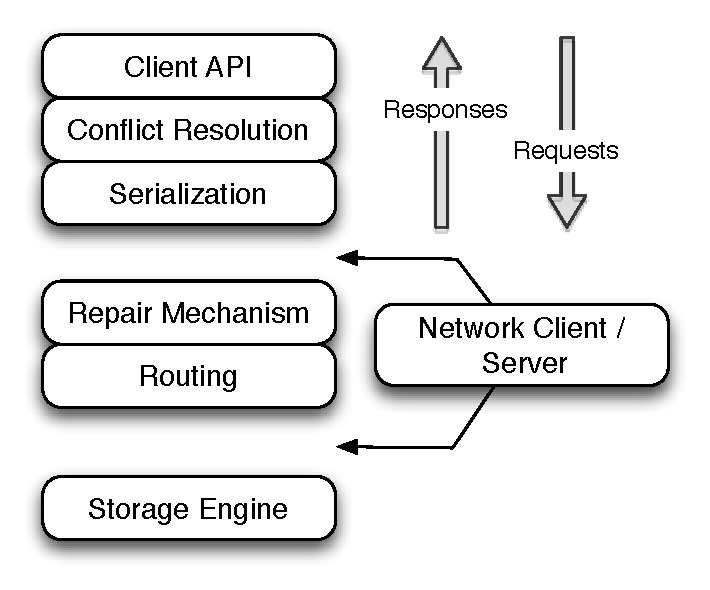
\includegraphics[scale=0.55]{images/arch.pdf}
  \caption{\projectname{} architecture containing pluggable and interchangable modules for a single client and server}
  \label{arch}
\end{figure}

\projectname{} has a pluggable architecture, as shown in Figure \ref{arch}. Each box represents a module, all of which share the same code interface. Every module has exactly one functionality, making it easy to interchange modules and place them in any order. For example, we can have the routing module on either the client side or the server side. Functional separation at the module level also allows us to easily mock these modules for testing purposes. For example, mocked storage engine backed by hash map for unit tests. 

Most of our modules have been motivated from the original Dynamo paper. Starting from the top our client has a simple $get$ and $put$ API. Every tuple is replicated for availability, with each value being versioned with a vector clock~\cite{lamport}. Conflicts during updates for read-write stores are resolved at the application level by the next module. This resolution problem does not apply for read-only stores since \projectname{} updates all the replicas of a key in a store at once, keeping them in sync. Similarly the `repair mechanism' layer, consisting of hinted handoff and read repair, is used only by read-write stores to bring the data back to a consistent state. 

The `routing' module deals with partitioning as well as replication. Our partitioning scheme is similar to Dynamo's, where-in \projectname{} splits the hash ring into equal size `partitions' and then assigns them to nodes. This ring is then shared with all the stores, i.e. changes in the mapping require changes to all the stores. Now to generate the `preference list' (list of node ids where the replicas will be stored), we first hash the key to a range belonging to a partition and then continue jumping the ring clockwise to find $N$-1 other partitions belonging to different nodes. 

The last module, i.e. the pluggable storage layer, has the same $get$ and $put$ functions, along with the ability to stream data out. Being able to iterate over all tuples in a store has proved to be very helpful during debugging of data. Besides running the above stack, every node also runs a service which allows the execution of following administrative commands - add / delete store, stream data out and trigger read-only store operations. 

\begin{figure}
  \centering
    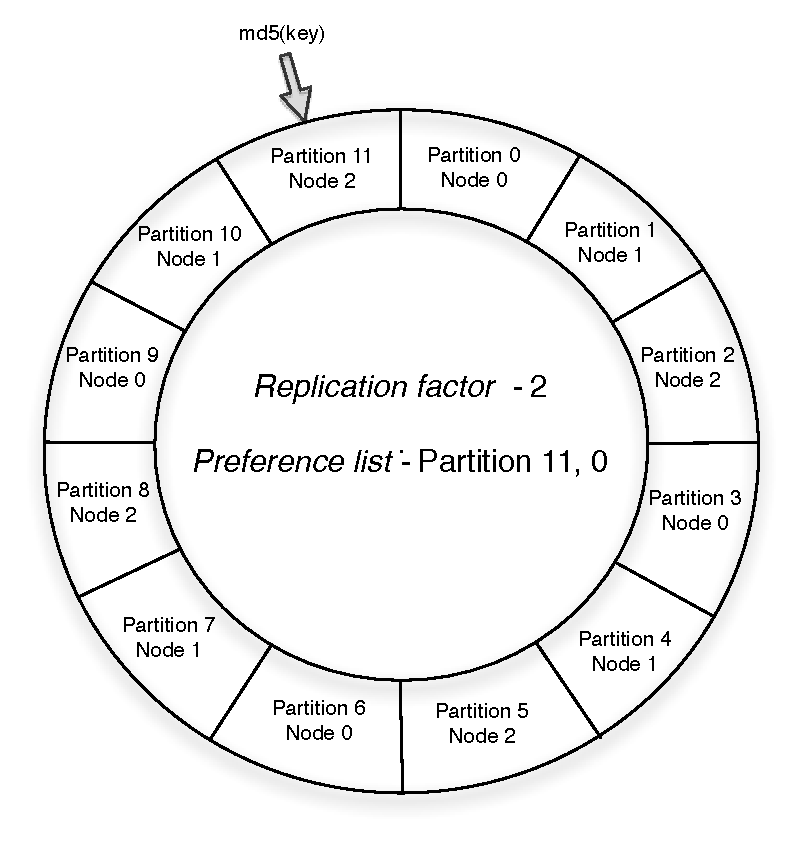
\includegraphics[scale=0.40]{images/hash.pdf}
  \caption{Simple hash ring cluster topology for 3 nodes and 12 partitions. The preference list for the key hashing to partition 11 for a store with replication factor of 2 is [ 11, 0 ]}
  \label{hash}
\end{figure}

\begin{figure}
  \centering
    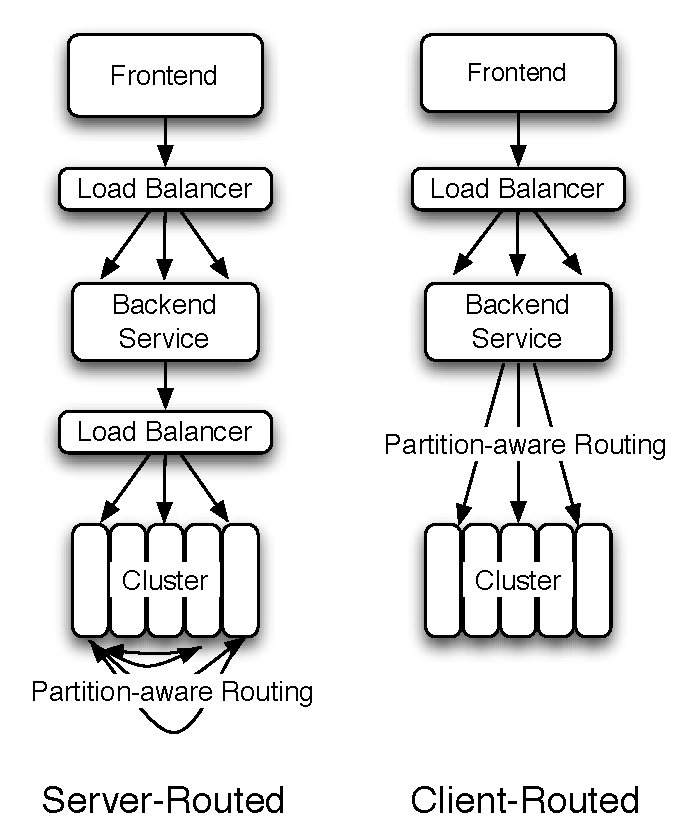
\includegraphics[scale=0.45]{images/fullstack.pdf}
  \caption{Two ways to use \projectname{} clusters in a website stack}
  \label{fullstack}
\end{figure}


\noindent 
Now that we know the individual components, let us look at how \projectname{} is being used inside the complete \linkedin{} stack. As shown in Figure, \ref{fullstack} \projectname{} supports two routing modes --- server side and client side routing. Client side routing requires an initial `bootstrap' step where-in it retrieves the metadata required for routing (cluster topology and store definitions metadata) by load balancing to a random node. Once the metadata has been retrieved the client gets the benefit of doing one less hop compared to server side routing since it knows exactly where the replicas for a key are. This is beneficial from a latency as well as throughput perspective since there are less number of services acting as bottlenecks. The disadvantage of client side routing is that it makes the client side code-base large because of the extra routing and replication logic. Also, as we'll further explain in Section~\S\ref{sec:read_only:data_cycle:rebalancing}, it also makes rebalancing of data complicated since the \projectname{} nodes now need a mechanism to update the cluster topology metadata on the live clients. 


% ========================== READ-ONLY-STORAGE ENGINE  ==========================================

\section{Read-only extensions}
\label{sec:read_only}

Before we started writing our own custom storage engine we decided to
evaluate currently available storage engines, MySQL and BDB, to see 
if they could fit our bulk loading use-case. Our criteria for success 
was the ability to bulk load data as fast as possible with minimum 
disk space overhead while still serving live traffic.
 
We started by evaluating the various storage engines provided by
MySQL. The na\"ive approach of multiple insert statements is
problematic as every statement results in an incremental change to the
underlying index structure---in this case, a B$^{+}$ tree---which in
turn results in many disk seeks. To solve this problem, MySQL provides
a \sql{LOAD DATA} statement that tries to bulk update the underlying
index, but this requires a lock of the entire table if the MyISAM
storage engine is used. This statement works for InnoDB which instead
supports row-level locking, but comes at the expense of substantial 
disk space overhead for every tuple. Also to achieve MyISAM-like bulk 
loading performance, InnoDB prefers data ordered by primary key.

Another solution to solve the above problem is to bulk load into a 
different table on the same cluster and use views on the client side to 
transparently swap to the new table. We attempted this with MyISAM 
storage engine, opting to skip InnoDB due to the huge space requirements.
This approach solves the locking problem but still hurts serving 
latency due to pressure on shared CPU and memory resources.  

We next tried completely offloading the index construction to another
system as building the index on the serving system has isolation
problems. To do so, we leveraged the fact that MyISAM allows copying 
of database files from another node into a live database directory; 
thereby automatically making it available for serving. 
We built a separate cluster where-in we would bulk load and then eventually 
copy the data over to the live cluster, but this requires an extra 
maintenance cost of a separate MySQL cluster with exactly the same number 
of nodes as the live one. Further, the lack of ability to load compressed 
data directly makes this process more time consuming, as the data is copied 
multiple times between nodes: once as a flat file to the bulk load cluster, 
then the internal copy during the \sql{LOAD} statement, and finally the 
raw data copy to the actual live database. 

The previous solution is not ideal due to its dependency on the
redundant MySQL servers, which makes the complete process prone to
failure downtimes. Instead, what if we could use the inherent fault
tolerance and parallelism of Hadoop and build individual node /
partition level data stores which could be pulled over by
\projectname{} for serving? The large-scale adoption of HDFS~\cite{hdfs}
 as the data sink for ETL scenarios makes it an ideal location to 
act as our source of data.
So the next attempted approach was to use Hadoop and a good single
node high performance storage engine to generate smaller data
stores in parallel. That is, a Hadoop job reads data from a source in
HDFS, re-partitions on a per node basis, and finally writes the data
to individual stores (for example, BDB) on the local filesystem in the
reducer phase. The number of reducers were equal to the number of
nodes, but could have easily been further split on a per partition
basis. This data is then read from the local filesystem and copied
onto HDFS from where it can be read by \projectname{}. The benefits of
this approach is that it leverages Hadoop's fault tolerance to build
the indexes offline, but it suffers from an extra copy from the local
file system the reducer nodes to HDFS---which can become a real
bottleneck with terabytes of data. 

From the above experiments we came to the conclusion that we required
our own custom storage engine. Our new custom storage engine, along
with its complete pipeline, should have the following properties. 
\begin{compactitem}
\item \emph{No performance impact on live requests}. The incoming
requests to the live store must not be impacted during the data load.
There is a tradeoff between modifying the current index on the live
server and finishing the bulk load as fast as possible, but that can
increase I/O and hurt performance. As a result, we completely rebuild
the index offline and also throttle the fetches. 
\item \emph{Fault tolerance and scalability}. Every step of the data
load pipeline should be able to handle failures. Hadoop, with its
ability to deal with failures, is used as the computation layer for
building the index. Similarly, HDFS's replication provides
availability for our data. Finally \projectname{} is used as the 
serving layer, providing fault tolerance with tuple level replication. 
All of these systems also easily scale horizontally due to
their already existing support for expansion without downtime. 
\item \emph{Rollback}. The general trend we notice in our business
that data is treated more like code: incorrect or incomplete data
could have been due to algorithm changes or source data problems. 
In such scnearios running a long batch load job to re-populate new
correct data is not acceptable. So to minimize the time in error, 
our storage engine must support very fast rollback to the previous 
good state.
\item \emph{Handle large data-sets}. Hadoop has successfully help
scale out data generation at commodity prices feasible.
This coupled with the rise of machine learning at internet companies 
leads to large data sets and opportunities to run potentially complex 
algorithms on them as a core production use case. Combination of 
the above two has led to large, cheap production of data which can 
be used as part of the product. Classic example of this for social 
networks includes storing relationships between pair of users,
or between users and an entity. When dealing with millions of users, 
this pairs data can easily reach billions of tuples, motivating
our storage engine to have support for TBs of data and perform 
well under large ratios of data to RAM ratio.
\end{compactitem}

Our data deployment pipeline consists of a new storage engine that
is built in Hadoop (\S\ref{sec:read_only:storage_format}), versioned
for rollback (\S\ref{sec:read_only:versioning}), and deployed. We
finally conclude by explaining how it fits into the complete data 
cycle along with some real world production scenarios and
how we dealt with it. 

% ========================== READ-ONLY-STORAGE ENGINE  - STORAGE FORMAT ==========================================

\subsection{Storage format}
\label{sec:read_only:storage_format}

Many storage formats try to build data structures that keep the data
memory-resident in the process address space, ignoring the effects of
the operating system's page cache. The several orders of magnitude 
latency gap between the page cache and disk means the only real 
performance benefit by maintaining our own structure is for elements 
already in the page cache. In fact, this custom structure may even 
start taking memory away from the page cache. Rather, this motivated 
the need of our storage engine to exploit the page cache instead of 
maintaining our own complex data structure. Since our data is immutable, 
\projectname{} memory maps the entire index into the address space. 
Further, since \projectname{} has been written in Java and runs on 
the JVM, delegating the memory management to the operating system 
eases garbage collection tuning.

\begin{figure}
  \centering
    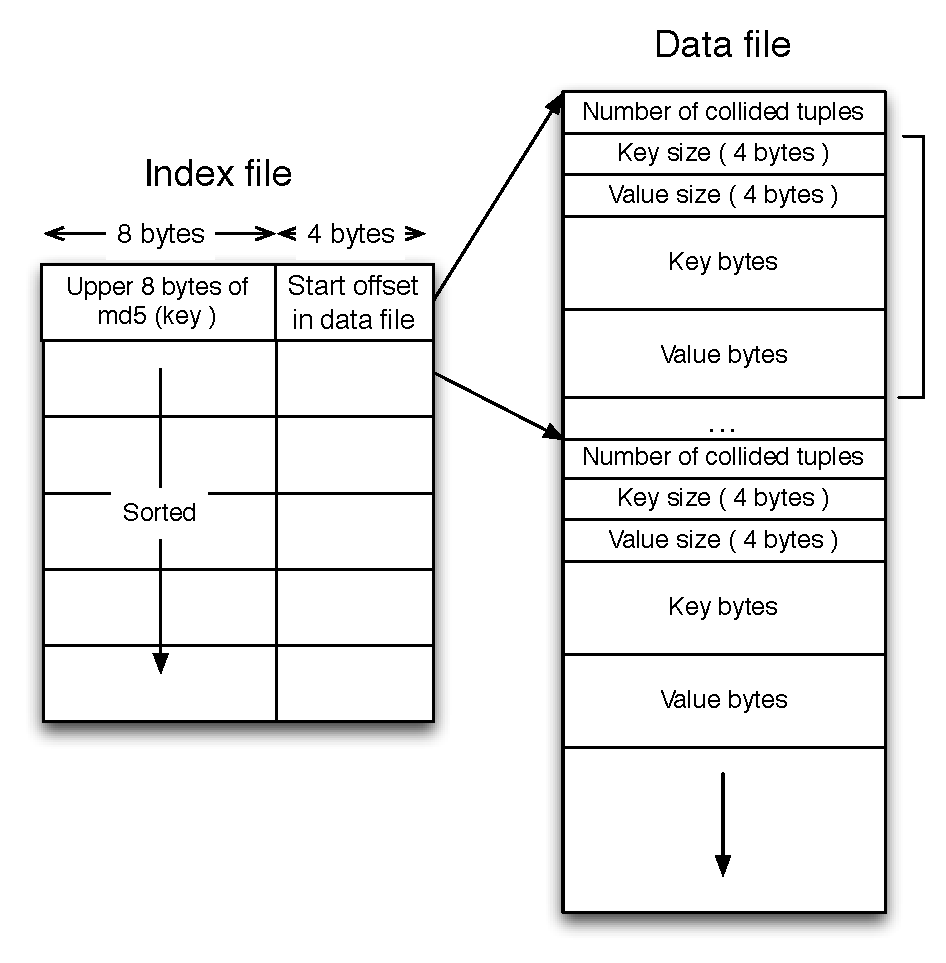
\includegraphics[scale=0.45]{images/storage_format.pdf}
  \caption{Read-only data is split into multiple chunks. A chunk contains an index and data file. The diagram shows the data layout in these files.}
  \label{storage_format}
\end{figure}

To take advantage of the parallelism in Hadoop, we split the data, 
destined for a particular node, into multiple chunk buckets, 
which in turn are split into multiple chunk files. Generation of 
multiple chunks file can hence be done independently and in parallel. 
A chunk bucket is defined by the primary partition id and replica type,
thereby giving it a unique identifier across all nodes. For example the key in 
Figure~\ref{hash} would fall into buckets~11\_0 (on node~2) and 
11\_1 (on node~0). Table~\ref{tab:node_to_chunk} summarizes the
various chunk buckets for a store with replication factor 2 and cluster
topology as defined in Figure~\ref{hash}. Our initial design 
had started with the simpler scheme of having one bucket per node 
(i.e. multiple chunks stored on a node with no knowledge about partitions), 
but this smaller granularity is necessary to aid in rebalancing~(\S~\ref{sec:read_only:data_cycle:rebalancing}).

Every chunk bucket contains multiple chunk files, count of which is
set on the Hadoop side. A chunk is a pair of data and 
index file. We have set a standard naming convention for all 
our chunk files - 
$\text{\emph{partition id}}\_\text{\emph{replica
id}}\_\text{\emph{chunk id}}.\{\text{data},\text{index}\}$ where
\emph{partition id} is the id of the primary partition and
\emph{replica id} is a number between 0 to $N-1$. 
Figure~\ref{storage_format} shows the structure of the storage
engine's data and index files. 

\begin{table}
\begin{center}
    \begin{tabular}{ | c | c | }
    \hline
    Node Id & Chunk buckets \\ \hline
    0 &  0\_0, 3\_0, 6\_0, 9\_0,      2\_1, 5\_1, 8\_1, 11\_1	\\
   1 &   1\_0, 4\_0, 7\_0, 10\_0,      0\_1, 3\_1, 6\_1, 9\_1		\\
   2 &    2\_0, 5\_0, 8\_0, 11\_0,    1\_1, 4\_1, 7\_1, 10\_1		\\
\hline
    \end{tabular}
\end{center}
 	\caption{Every \projectname{} node is responsible for chunk buckets based on the partitions and replica type. This table shows the node id to chunk bucket mapping for the cluster topology defined in Figure~\ref{hash}}
 	\label{tab:node_to_chunk}
\end{table}

The index file is a compact structure containing the sorted upper
8~bytes of the MD5 of the key followed by the 4~byte offset of the
corresponding value in the data file. This simple sorted structure
allows us to easily leverage Hadoop's ability to return sorted data
in the reducers. Further, preliminary tests also showed that the
index files were generally order of magnitude smaller than the data
files and hence, could safely fit into the page cache.

An interesting optimization is that the full 16 bytes of the MD5 of
the key is not necessary. We had initially started by using the full
MD5 signature, but over time we noticed multi-tenant performance
problems: stores were stamping on each others pages in the page cache.
To alleviate this problem, we needed to cut down on the amount of data
being memory mapped, which can be achieved by reducing the available
key-space and accepting collisions in the data file. 

Our optimization proceeded as follows and can be mapped to the classic
birthday paradox: if we want to retrieve $n$ random integers from a
uniform distribution of range $[1, x]$, the probability that at least
2 numbers are the same is:
\begin{equation}
1 - e^{\frac{-n(n-1)}{2x}}
\end{equation}
Mapping this to our scenario, $n$ is generally our 120 million member
user base, while the initial value of $x$ is $2^{128} - 1$ (16 bytes
of MD5). The probability of collision in this scenario was close to 0.
A key-space of 4 bytes (i.e. 32 bits) yields an extremely high
collision probability of:
\begin{equation}
1 - e^{\frac{(-120*10^{6} * (120*10^{6} - 1)}{2 * (2^{32} - 1)}} \sim 1
\end{equation}
Instead, a compromise of 8 bytes (i.e. 64 bits) produces:
\begin{equation} 
1 - e^{\frac{(-120*10^{6} * (120*10^{6} - 1)} { 2 * (2^{64} - 1 )}} < 0.0004
\end{equation}
The probability of more than one collision is even smaller. Thus, by
decreasing the number of bytes of the MD5 of the key we were able to
cut down the index size by 40\%, thereby making our clusters more
multi-tenant. The size of the keys-space is an optional parameter the
admin may set depending on the semantics of the data. Unfortunately,
this came at the expense of us having to save the keys in the data
file to use for lookups and handle the rare collisions in the data
files.

The data file is similarly a very highly packed structure where we
store the number of collided tuples followed by a set of collided
\emph{(key size, value size, key, value)} list. The important thing to
remember here is that we store the raw key bytes instead of the MD5-ed
key bytes in order to do a comparison during reads. 

% ========================== READ-ONLY-STORAGE ENGINE  - VERSIONING ==========================================

\subsection{Versioning of data}
\label{sec:read_only:versioning}

One of our requirements was the ability to rollback the data. The
above chunk files need to be stored in a layered format so as to allow
rollback. Every time a new copy of the complete data-set is created,
the system needs to demote the previous copy to an older state.

Every store is represented by a directory which then contains various
``versions'' of the data. Since the data in all the version
directories, except the serving one, are inactive we are not affecting
the page cache usage and hence the latency. Also since nowadays disk
space is cheap and provides very fast sequential writes compared to
random reads, keeping these previous copies(number of which is
configurable) is beneficial for quick rollback. Every version folder
(named \term{version-\emph{no}}) has a configurable number associated
with it, which should increase with every new fetch. An example of the
version number is the timestamp of push. 

Deploying a new data version is as simple as starting a new version
folder, changing the symbolic link to the latest data and swapping the
data in. Similarly, a rollback requires changing the symbolic link to a 
previous version folder and swapping the data in. 

% ========================== READ-ONLY-STORAGE ENGINE  - CHUNK GENERATION ==========================================

\subsection{Chunk generation}
\label{sec:read_only:chunk_generation}

Construction of the chunk files for all \projectname{} nodes is a
single MapReduce job; the pseudo-code representation is shown in
Figure~\ref{fig:mapreduce-chunk-generation}.

\begin{algorithm}
\scriptsize
\DontPrintSemicolon
\SetKwFunction{mapper}{map}
\KwIn{K: raw key}
\KwIn{V: raw value}
\SetKwBlock{Map}{map(K,V)}{end}
\SetKwBlock{Partitioner}{partition(K,V): int}{end}
\SetKwBlock{Reducer}{reduce(K,Iterator$<$V$>$ Iterator)}{end}

\Map{
	K' $\leftarrow$ MakeKey(K,V)\;
	V' $\leftarrow$ MakeValue(K,V)\;
	Replica Id $\leftarrow$ 0\;
	KOut $\leftarrow$ TopBytes(MD5(K'),8)\;
	\ForEach{Partition Id $\in$ PreferenceList(MD5(K'))}{
		Node Id $\leftarrow$ PartitionToNode(Partition Id)\;
		emit(KOut, [Node Id, Partition Id, Replica Id, K', V'])\;
		Replica Id $\leftarrow$ Replica Id + 1\;
	}
}

\BlankLine
\KwIn{K: Top 8 bytes of MD5 of Spock key}
\KwIn{V: [Node Id, Partition Id, Replica Id, Spock key, Spock value]}

\Partitioner{
	Chunk Id $\leftarrow$ TopBytes(MD5(K'),Size(int)) \% Num Chunks\;
	Bucket Id $\leftarrow$ V.Partition Id * Replication Factor + V.Replica Id\;
	\Return{Bucket Id * Num Chunks + Chunk Id}
}


\BlankLine
\KwIn{K: Same as partitioner} 
\KwIn{V: Same as partitioner} 

\Reducer{
	WriteIndexFile(K)\;
	WriteIndexFile(Position)\;
	WriteDataFile(Iterator.size)\;
	\ForEach{V $\in$ Iterator} {
		WriteDataFile(Size(V.K'))\;
		WriteDataFile(Size(V.V'))\;
		WriteDataFile(V.K')\;
		WriteDataFile(V.V')\;
	}
}
\BlankLine
\caption{MapReduce pseudo-code used for chunk generation}
\label{fig:mapreduce-chunk-generation}
\end{algorithm}

The Hadoop job consists of a simple MapReduce job which takes as its
input the number of chunk files per chunk buckets, cluster topology, 
store definition and the input data location on HDFS and then 
takes care of replication and partitioning, finally emitting the 
data into separate node based folders. 

This is achieved by partitioning the data depending on the routing
strategy in the mapper phase; redirecting the key to the correct reducer 
in the partitioner phase and finally writing the data to a single
chunk (i.e. a data and index file) in the correct node folder in the
reducer phase. Due to Hadoop's generic \term{InputFormat} mechanics, any source data
can be converted to \projectname{}'s serialization format. The mapper
phase emits the upper 8~bytes of MD5 of the \projectname{} key
$N$~times as the map phase key with the map phase value equal to a
grouped tuple of node id, partition id, replica id and the raw
\projectname{} key and value. 

The custom partitioner then generates the chunk id within a chunk
bucket from this key. Since there is a fixed number of chunks on a 
per partition-replica basis, the chunk id is generated with a 
simple mod of the number of chunk files per chunk bucket. 
It then uses the partition id, replication factor of the store and 
the chunk id to route the key to the correct reducer. 

Finally, every reducer is responsible for a single chunk, 
meaning that by having more chunks, once can increase
the parallelism during the build phase. Since Hadoop automatically
sorts the data based on the key, the process receives data in the
order necessary for the index file and can a simple append 
to the index and data file on HDFS with no extra processing required.
The data layout on HDFS is a directory on a per \projectname{} node
basis, with the nomenclature of \term{node-\emph{id}}.

% ========================== READ-ONLY-STORAGE ENGINE  - SEARCH ==========================================

\subsection{Retrieval}
\label{sec:read_only:search}

To find a key, the client generates the preference list and directs
the request to the individual nodes, depending on $R$. 
The following is a sketch of the algorithm to find the data once it
reaches a particular node.

\begin{compactenum}
  \item Calculate the MD5 of the key
  \item Generate the (i) primary partition id (ii) replica id (the replica being
searched when querying this node) and (iii) chunk id (the first 4 bytes of
the MD5-ed key modulo the number of chunks in a bucket)
  \item From the store's folder, find the corresponding chunk file 
(data and index) with the above 3 variables.
  \item Perform a binary search using the top 8~bytes of the MD5-ed
key as the search key in the index file. This is easy, as there are
fixed space requirements for every key (12 bytes: 8 bytes for key and
4 bytes for offset), thereby not requiring any internal pointers
within the index file. For example, the data location of the $i$-th
element in the sorted index is simply a jump to
the offset $12 \cdot i + 8$.  
  \item Read the corresponding data location from the index file
and jump to the location in the data file. Iterate through any 
potential collided tuples, comparing keys, and returning the 
corresponding value on key match. 
\end{compactenum}

The most time consuming step is search in the index file. A binary
search in an index of 1~million keys can result in around 20~key
comparisons, which means if the index file is not cached, there will be
20~disk seeks to read one value. As a small optimization, while
fetching the files from HDFS, \projectname{} transfers the index files
after all data files to aid in keeping the index files in the OS page
cache.

Rather than binary search, another retrieval strategy for sorted disk
files is interpolation search~\cite{manolopoulos}. This search
strategy uses the key distribution to predict the approximate location
of the key, rather than halving the search space on every iteration.
Interpolation search works well for uniformly distributed keys,
dropping the search complexity from $O(log~N)$ to $O(log~log~N)$. This
helps in the un-cached scenario by reducing the number of disk seeks.

We have also looked into other strategies like Fast and Pegasus. As
proved in \citet{manolopoulos}, most of these are better suited for
non-uniform distributions. As MD5 (and its sub-sets) provide a fairly
representative uniform distribution, there will be minimal speedup
from these techniques.

% ========================== READ-ONLY-STORAGE ENGINE  - COMPLETE DATA CYCLE ==========================================

\subsection{Complete data cycle}
\label{sec:read_only:data_cycle}

Figure \ref{cycle} shows the complete data cycle that eventually
results in new data being swapped into a \projectname{} store. 

\begin{figure}
  \centering
    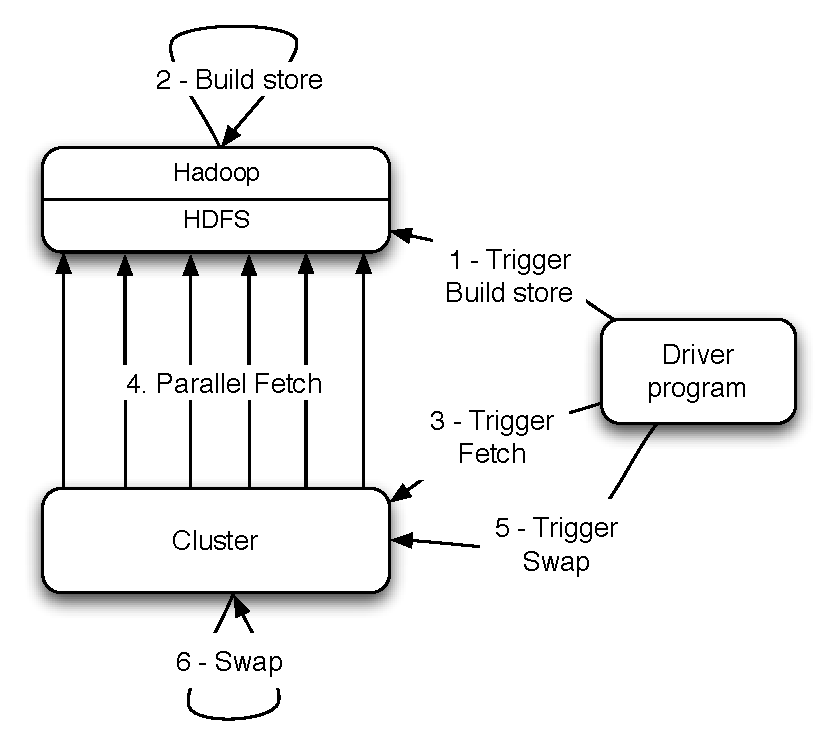
\includegraphics[scale=0.60]{images/cycle.pdf}
  \caption{Steps involved in the complete read-only data cycle. The components involved include Hadoop, HDFS, \projectname{} and a driver program co-ordinating the full process.}
  \label{cycle}
\end{figure}

The initiator of this complete fetching and swapping of new data is a
standalone driver program, which starts by triggering the Hadoop job
described in Section~\S\ref{sec:read_only:chunk_generation}. This job
generates the data on a per node basis and stores it into HDFS. While
streaming the data out onto HDFS, the system also calculates a
checksum on a per node basis by storing a running MD5 on the
individual MD5s of all the chunk files. 

Once the Hadoop job is complete, the driver triggers a fetch request
on all \projectname{} nodes. This request is received by each node's
``administrative service,'' which then initiates a parallel fetch for
its respective node folder. While the data is being streamed from
HDFS, the checksum is validated with the checksum from the build step.
\projectname{} uses a pull model, rather than a push model, as it allows
throttling of this fetch in case of latency spikes.

After the data is available on each respective node, \projectname{} must swap
the new data-set with the older version. Finally after the fetch is
complete, the driver triggers a swap operation on all nodes, which is
co-ordinated via a read-write lock in the storage engine. Each node
closes its current set of chunks, open its new set of chunks, and
memory maps the new index. On a single node, this complete 
operation takes around 0.012 ms on average with the worst swap time of 
around 0.050 ms. This is because no data reads are required for the 
swap. To provide global atomic semantics, the driver ensures that 
all the nodes have successfully swapped their data; rolling back if 
any swaps have failed.

% ========================== READ-ONLY-STORAGE ENGINE  - COMPLETE DATA CYCLE - SCHEMA CHANGE ==========================================

\subsection{Schema upgrades}
\label{sec:read_only:data_cycle:schema_upgrades}

There are bound to be changes to the underlying data model; a common
example of this is if a product wants to add a new dimension to their
value. \projectname{} supports the ability to change the schema of the
key and value without downtime: since the data is static and the
system does a full refresh, the schema can easily be changed. For the
client to transparently handle this change, the system encodes a
special version byte in the binary JSON serialization format. This
same version information is saved in the stores' metadata, which
clients pick up during bootstrapping. The clients maintain a mapping
from version-id to corresponding schema, so if a data fetch introduces
a new schema, during the read the client will toggle the right version
id and pick up the corresponding schema. Similarly, during rollback,
the client toggles to an older version of schema and is able to read
the data with no downtime. 

% ========================== READ-ONLY-STORAGE ENGINE  - COMPLETE DATA CYCLE - REBALANCING ==========================================

\subsection{Rebalancing}
\label{sec:read_only:data_cycle:rebalancing}

Over time as new stores get added to the cluster, the disk to memory
ratio increases beyond the initial capacity planning, resulting in
increased read latency. Our data being static, the na\"{i}ve
approach of starting a new larger cluster, re-pushing the data, and
switching clients does not work as it requires massive co-ordination
of 100+ clients communicating with 100+ stores.

This motivates the need to have a feature to transparently and 
incrementally add capacity to the cluster indepedent of the data pushes. 
The rebalancing feature allows us to add new nodes to a live cluster without 
downtime. This feature was initially written for the read-write stores 
but easily fits into the read-only cycle due to the static nature 
of the data. Our smallest unit of rebalancing is a partition. In 
other words, addition of a new node translates to giving the ownership 
of some partitions to it. The rebalancing process is run by a tool that 
co-ordinates the full process. The following are the steps that
are followed during the addition of a new node. 

\begin{compactenum}
\item Provide the rebalancing tool with the future cluster topology
metadata.

\item Using the future cluster topology metadata, generate list of all
primary partitions that need to be moved

\item Do the following steps for every batch of primary partitions,
which allows moving the partition in small batches so as to make the
process checkpoint-able without having to re-fetch too much data. 

\begin{compactenum}

\item Generate intermediate cluster topology metadata which is current
cluster topology with changes in ownership of batch of partitions
moved

\item Use intermediate cluster topology metadata to generate a set of
steps that need to be run to finish rebalancing. In this process,
\projectname{} must take care of all the secondary replica movements that might
be required due to the primary partition movement. This plan is a set
of donating node id and stealing node id pairs along with the chunk
files being moved. 

\item Initiate asynchronous processes (through the administrative
service) on all the stealer nodes which then start stealing chunk
files from their corresponding donor nodes. These nodes to go into a
``rebalancing state'' and are thereby do not take any new data.
			
Here it is important to note that the granularity of the bucket
selected makes this process as simple as copying files. If buckets
were defined on a per node basis (i.e. have multiple chunks on a per
node basis), the system would need to iterate over all the keys on the
node and find the correct key set belonging to the moving partition,
then merging this key set with the live serving index on the stealer
node's end. 

\item Once the fetches have completed, the rebalancing tool updates
the intermediate cluster topology on all the nodes while also doing an
atomic swap of data on the stealer and donor nodes. 
			
This topology change information also needs to be propagated to all
the upper services using client side routing. \projectname{} propagates
this information as a lazy process where-in the clients still use the
old metadata. If they contact a node with a request for a key in a
partition which the node is no more responsible the node sends a
special exception, which results in a re-bootstrap step along with a
retry of the previous request.

\end{compactenum}

\end{compactenum}

The rebalancing tool has also been designed to handle failure
scenarios elegantly. Failure during a fetch is not a problem since no
new data has been swapped. However, failure during the swap requires a
rollback of the cluster topology to the last good cluster topology
while also rolling back the data on the successful nodes. 

Table~\ref{tab:new_node_to_chunk} shows the new chunk mapping when a
new node is introduced to cluster with the same hash ring as Figure
\ref{hash}. This node is now responsible for partition 3. Table 
\ref{tab:rebalance_plan} shows the simple plan that would be generated
during rebalancing.
 
\begin{table}
\begin{center}
    \begin{tabular}{ | c | c | }
    \hline
    Node Id & Chunk files \\ \hline
    0 &  	0\_0, 6\_0, 9\_0,      			5\_1, 8\_1, 11\_1 			\\
   	1 &   	1\_0, 4\_0, 7\_0, 10\_0,      	0\_1, 3\_1, 6\_1,9\_1  		\\
   	2 &    	2\_0, 5\_0, 8\_0, 11\_0,    	1\_1, 4\_1, 7\_1, 10\_1		\\
   	3 &   	3\_0,                         	2\_1 						\\
\hline
    \end{tabular}
\end{center}
 	\caption{Node to chunk bucket mapping after addition of 4th node ( node id 3 ) to the existing cluster defined by ring in Figure~\ref{hash}}
 	\label{tab:new_node_to_chunk}
\end{table}

\begin{table}
\begin{center}
    \begin{tabular}{ | c | c | c | }
    \hline
    Stealer Node Id & Donor Node Id & Chunks to steal \\ \hline
    3 &  0 & 3\_0, 2\_1	\\
\hline
    \end{tabular}
\end{center}
\caption{Rebalancing plan generated for addition of new node in Table~\ref{tab:new_node_to_chunk}}
\label{tab:rebalance_plan}
\end{table}

